\documentclass[thesis.tex]{subfiles}

\begin{document}

% ----------------------------------------------------------
\chapter{Background} \label{chap:background}
% ----------------------------------------------------------
% Present the background
% ----------------------------------------------------------
In recent years there have been many proposed methods to use automated object tracking, segmentation, deep learning and artificially intelligence to produce a better, and cheaper health care system. Many of the methods used are state of the art systems within the fields of deep learning. One requirement for such a system to work in reality is a good flow of data. Ideally all the data should be labeled by a doctor before it is used for training deep neural networks but this is rarely the case. The method which we propose takes advantage of this unlabeled data which is more readily available.

In this chapter we will present the necessary background and related works to understand how such a semi supervised model can be built. This will be covered over two main parts; one where we go through the related background and works to understand the medical aspect of this topic and the other will cover the technical use of deep learning in mission-critical fields such as the medical domain.

We begin with the digestive system and how it operates to aid the human body with digestion of food. Next we will cover disease detection by using various types of endoscopes. We will look at how the current state of lesion detection and how it could be improved by using deep learning. 

In the next part will focus on deep learning and its various architectures and building blocks. To fully understand this we need to have a look at its inner workings and output. We begin with looking at a basic three layer neural network and build from there up to CNNs and some of the most advanced architectures most recently proposed. This will give a good understanding of how and why we use deep learning to classify medical images.


% ----------------------------------------------------------
\section{Medical scenario} \label{sec:medical_scenario}
% ----------------------------------------------------------
Here we will go through the medical aspect of our problem statement, beginning with the anatomical explanation of the digestive tract. 


\subsection{Colon cancer} \label{sec:colon_cancer}
% ----------------------------------------------------------
% what are colon cancer, and other lesions in GI tract 
% doing to the effected patients, what are death rates
% and the cost to society etc
% ----------------------------------------------------------


\subsection{The digestive system}  \label{sec:the_digestive_system}
% ----------------------------------------------------------
% what to look for when analyzing videos from the digestive system
% ----------------------------------------------------------
To detect irregularities in the digestive system (Figure \ref{fig:digestive_system}) is a difficult and time-consuming task. To classify irregularities correctly and precisely require expert knowledge. Fortunately we have access to data which already has been labeled by trained professionals that we will use in this project.

The most common way of screening patients is with a endoscope. When this tool is used by a professional some of the irregularities that can be spotted are; \textit{Colon polyp}, \textit{Colorectal Cancer}, \textit{Ulcerative Colitis}, \textit{Crohn's Disease}, \textit{Familial adenomatous polypsis}, \textit{Diverticulosis} and \textit{Diverticula Bleeding}. 

These diseases have varying patterns and while some can be easy to split apart, some are more similar in pattern. While for an untrained eye it can be easy to spot that something is wrong it is very difficult to describe with words what that might be or even harder to write a program to detect the correct characteristic features of the disease. This is why we rely on having good amount of labeled data for this project to work. For increased accuracy we may have to look closer at a couple of diseases. Preferably two irregularities that both have different characteristics and lots of labeled training data.

\begin{figure}[ht] % fig:digestive-system
  \begin{center}
    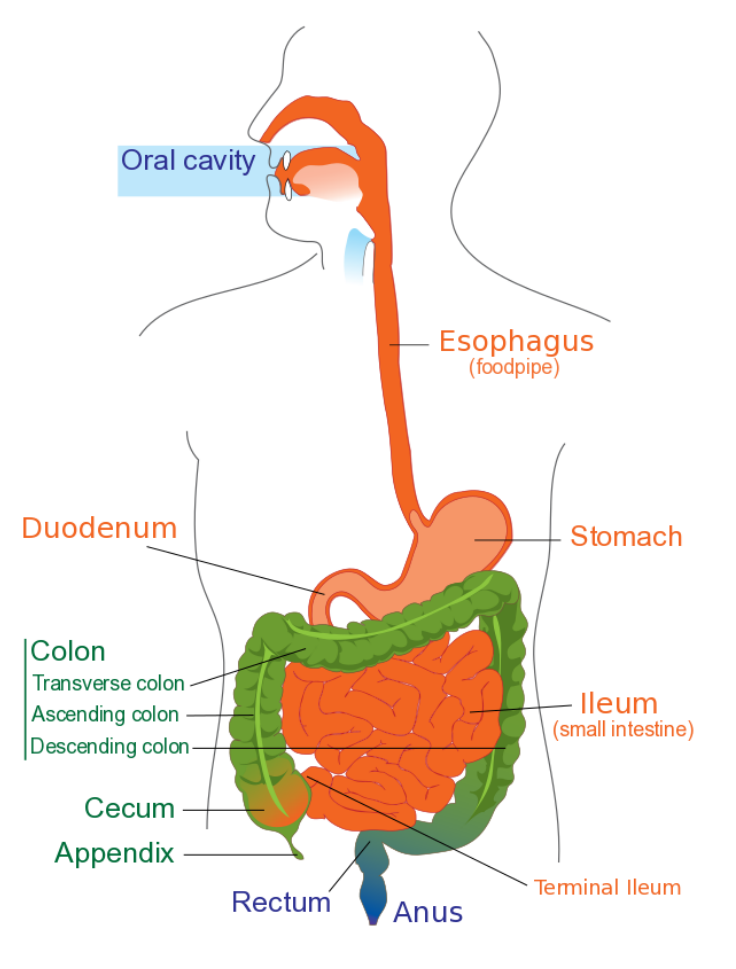
\includegraphics[width=0.5\textwidth]{digestive-system}
    \caption[An overview of the terms used to describe the digestive system]{An overview of the terms used to describe the digestive system\footnotemark.}
    \label{fig:digestive_system}
  \end{center}
\end{figure}

\footnotetext{
\text{By Mariana Ruiz, edited by Joaquim Gaspar. Released into public domain by author.} \newline
\url{https://en.wikipedia.org/wiki/File:Digestive_system_diagram_edit.svg}
}


\subsection{Traditional Endoscopy}
% ----------------------------------------------------------


\subsection{Wireless Capsule Endoscopy}  \label{sec:wireless_capsule_endoscopy}
% ----------------------------------------------------------
% general info about WCE, some history etc
% ----------------------------------------------------------
The basic technology behind the modern endoscope was developed in the early 1950s by English physicist Harold Hopkins and his student Narinder Kapany which let light travel through flexible pieces of glass, now known as optical fibers \cite{NewMethod54}.

Before the year 2000 the only option you had to visualize the food pipe, stomach, duodenum, colon and terminal ileum (see Figure \ref{fig:digestive_system} for details) was to use a fiber-optic endoscope, which is a tool with a relatively wide cable that is pushed into the bowel with as much as 50 000 optic fibers (as seen on Figure \ref{fig:fiber-optic-endoscopy}). These cables have to carry fiber optic bundles, water pipes, operations channel and control cables. Although these cables can be quite flexible there is a limit for how far they can advance into the small bowel. This method cause pain and discomfort for the patient, and there was a clinical need for an improved methods.

\begin{figure} % fig:fibre-optic-endoscope
  \begin{center}
    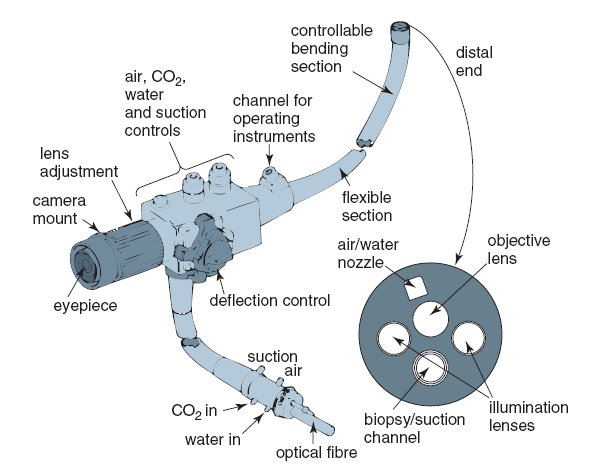
\includegraphics[width=0.7\textwidth]{fiber-optic-endoscope.jpg}
    \caption[Image of a fiber optic endoscope with explanation of different parts of the tool]{Image of a fiber optic endoscope with explanation of different parts of the tool\footnotemark.}
    \label{fig:fiber-optic-endoscopy}
  \end{center}
\end{figure}

\footnotetext{
\text{Image credit: Jacaranda Physics 1 2nd Edition © John Wiley \& Sons, Inc.}
}

That is why in the year \citeyear{WirelessCapsule00} \citeauthor*{WirelessCapsule00} developed a new type of video-telemetry capsule endoscope that was swallowable \cite{WirelessCapsule00}. It could travel through the entire digestive system because it had no external wires, fiber-optic bundles or cables of any sort. The capsule travels by peristalsis\footnote{Peristalsis is a radially symmetrical contraction and relaxation of muscles that propagates in a wave down a tube, in an anterograde direction.} through the gastrointestinal tract, which takes from 10 to 48 hours, and transmit images on a regular interval to receivers attached around the outside of the patients stomach for as long as the battery allows, usually in the range 6 to 8 hours. Two example images taken by WCE are presented in Figure \ref{fig:pillcam_examples}. By triangulating the signal strength and the location of the receivers taped on the body it is possible to roughly estimate the position of the capsule. This is however not very precise and can not tell us the rotation or direction of the capsule. Regardless, that information will not be available for us in this study as we only have access to the images themselves. Therefore we could implement an algorithm to predict which region of the digestive system the image is taken from (see section \ref{sec:mapping}).

\begin{figure} % fig:pillcam_examples (double figure)
  \centering
  \begin{subfigure}[b]{0.4\linewidth}%
    \centering
    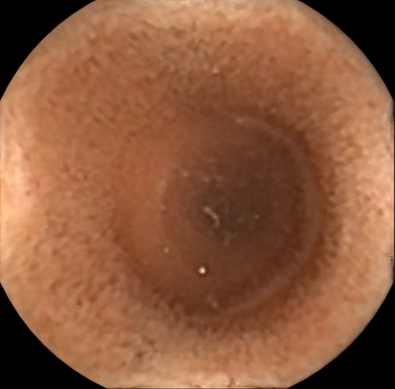
\includegraphics[width=\linewidth]{pillcam_small_intestine}%
    \caption{Small Intestine}%
    \label{fig:pillcam_small_intestine}%
  \end{subfigure}%
  \quad
  \begin{subfigure}[b]{0.4\linewidth}%
    \centering
    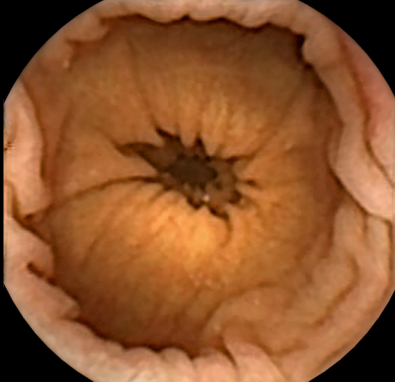
\includegraphics[width=\linewidth]{pillcam_colon}%
    \caption{Colon}%
    \label{fig:pillcam_colon}%
  \end{subfigure}%
  \caption[Images taken with WCE]{Images taken with WCE\footnotemark.}%
  \label{fig:pillcam_examples}%
\end{figure}%

\footnotetext{
\text{CC BY-SA 3.0 / Attribution to Dr.HH.Krause at English Wikipedia;} \newline
\url{https://commons.wikimedia.org/wiki/File:Normales_Colon.PNG} \newline
\url{https://commons.wikimedia.org/wiki/File:Dunndarm.PNG} %Dünndarm
}




% ----------------------------------------------------------
\section{Deep learning} \label{sec:deep_learning}
% ----------------------------------------------------------
As apposed to using regular optic-fiber endoscopy, it can be difficult to know the location and orientation of the capsule when it is traveling through the digestive system. In a paper by \citeauthor*{ClassifyingDigestive15} it is shown that by using Deep Convolutional Networks (DCNN) it is possible to classify the digestive organs in wireless capsule endoscopy with about 95\% classification accuracy on average \cite{ClassifyingDigestive15}.
The DCNN-based WCE digestive organ classification system is constructed of three stages of convolution, pooling and two fully-connected layers. This is illustrated in Figure 3 in the paper \cite{ClassifyingDigestive15}. The main steps of this convolutional neural network are described in detail in section \ref{convolutional_neural_network}.

\subsection{Imbalanced data}

\subsection{TensorFlow Framework} % ?? Perhaps add everything under framework/libraries?
%\subsection{Keras}
\subsection{Data pipeline} % ??


\subsection{Machine learning types} \label{sec:machine_learning_types}
% reinforcement learning, supervised, unsupervised and semi-supervised
% ----------------------------------------------------------
In deep learning it is common to differentiate between three types of machine learning models, supervised learning, unsupervised learning and reinforcement learning. In this section we will go through them and explain how they function and which use cases suites them best. In addition we will introduce a combination of supervised and unsupervised learning, called semi-supervised learning.

\subsubsection{Supervised learning} \label{sec:supervised_learnign}
% https://blogs.nvidia.com/blog/2018/08/02/supervised-unsupervised-learning/
The first category of machine learning is supervised learning. If you imagine yourself work under supervision of a leader or boss, it would mean someone is present and judging whether you are doing the correct work. Similarly to this, when a learning algorithm is under supervision is has a fully labeled dataset to work on; continuously updating the algorithm whether the answer is correct or wrong after every test.

Fully labeled dataset means that for every sample in the dataset, it is known what the true answer is to the problem at hand. Example if the dataset is images to classify you can think of it as having the correct answer written on the back of the image, but the algorithm will pick up the image front side up, and not look at the correct answer until after making a prediction.

%TODO reference to the image or create own?
\begin{figure}[h] % fig:supervised_machine_learning
  \begin{center}
    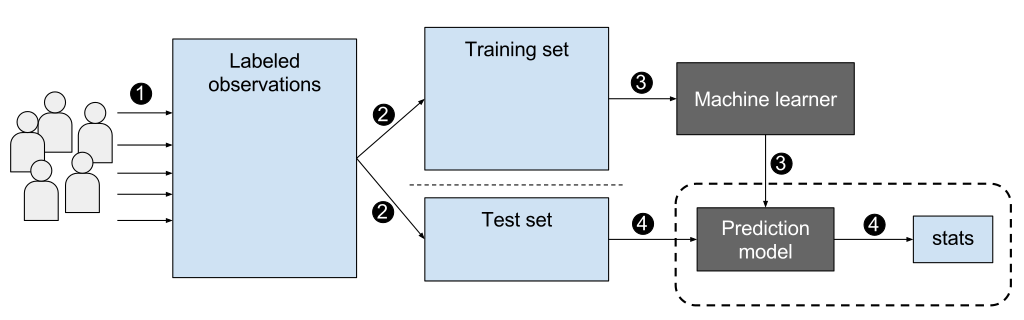
\includegraphics[width=0.7\textwidth]{supervised_machine_learning.png}
    \caption[Workflow of supervised machine learning.]{Workflow of supervised learning; 1. the dataset is labeled by observers; 2. the samples is split into training and test sets; 3. algorithm is learning on the training set; 4. checking the predictions on the 'unseen' test set to understand how the model performs.}
    \label{fig:supervised_machine_learning}
  \end{center}
\end{figure}

This method is best suited for classification problems and regression problems, where there is a set of available reference points or a ground truth with which to train the algorithm, but this is not always accessible, or too expensive to create.


\subsubsection{Unsupervised learning} \label{sec:unsupervised_learning}
% https://blogs.nvidia.com/blog/2018/08/02/supervised-unsupervised-learning/
Large, cleanly labeled datasets are not does not always easy to come by. And sometimes the answers we are looking for are not discrete, but discontinuous and hard to define. This is where unsupervised learning come in.

In unsupervised learning, the algorithm is handed non-labeled data without any instructions on what to do with it. It is the algorithms job to automatically find which features that best separates the data and find a structure within it.	An example of a problem well suited for unsupervised learning is; %TODO add example

Since the training data has not been reviewed by a human beforehand it is difficult to say with certainty how good the final model perform like it is with supervised learning.


\subsubsection{Reinforcement learning} \label{sec:reinforcement learning}



\subsection{How to evaluate a model}

\subsection{Performance metrics}

\subsection{Convolutional Neural Network} \label{convolutional_neural_network}
% write some general stuff about CNN's
% ----------------------------------------------------------
One of the most used neural networks for image classifcation is the Convolutional Neural Network (CNN). The model was first proposed by \citeauthor*{ImageNetClassification12} in \citeyear{ImageNetClassification12} \cite{ImageNetClassification12} where they trained a deep convolutional neural network and used it to classify 1.2 million high-resolution images in the ImageNet LSVRC-2010 contest into the 1000 different classes with top-1 and top-5 error rates of 37.5\% and 17.0\% which far surpassed all other models at the time. Next we will get into a bit of the details of a CNN.


\subsubsection{Convolution layer}
% ----------------------------------------------------------
The first step in a convolutional neural network is to extract features from the input image. This is done to preserve the relationship between pixels by learning image features using filters, or \textit{kernels}. As a result, the network learn filters that activate when it detects some specific patterns or features.

The convolution of \textit{f} and \textit{g} is written as $f*g$, and is defined as the integral of the product of the two functions after one (usually the filter) is reversed and shifted.

\begin{equation} % eq:convolution_func
  (f*g)(t) = \int_{-\infty}^{\infty} f(\tau) g(t-\tau) d\tau
  \label{eq:convolution_func}
\end{equation}


\subsubsection{Non Linearity (ReLU)}
% ----------------------------------------------------------
Rectified Linear unit function, known as simply ReLU, is an activation function represented by equation (\ref{eq:relu_func}). It sets all negative numbers to zero, by discarding them from the activation map entirely. In this way, ReLU increases the nonlinear properties of the decision function and thus of the overall network without affecting the receptive fields of the convolution layer.

\begin{equation} % eq:relu_func
    ReLU(x) = max(0, x)
    \label{eq:relu_func}
\end{equation}


\subsubsection{Pooling layer}
% ----------------------------------------------------------
Pooling layers are applied to reduce the number of parameters when the images are considerably large. Spatial pooling, or merely down sampling, reduces the dimensionality of each image but it keeps the important information. The most used down sampling is max pooling. It extracts the largest element from the rectified feature map and thus reduces computational complexity of the algorithm. In addition average pooling is also frequently used, this method computes the average value of the input map. The input-output model is denoted as:

\begin{equation} % eq:pool_func
  y_i = f(pool(x_i))
  \label{eq:pool_func}
\end{equation}


\subsubsection{Fully-connected layer}
% ----------------------------------------------------------
In a FC-layer every neuron in one layer is connected to every neuron in the previous layer. It is here the high-level reasoning is done. The activation function in the neurons is a \textit{sigmoid} or \textit{tanh} function.

\begin{equation} % sigmoid and tanh func
  f(z) = \frac{1}{1+exp(-z)} \quad \text{or} \quad f(z) = tanh(z) = \frac{e^{z} - e^{-z}}{e^{z} + e^{-z}}
\end{equation}

At the end of FC-layer we have an activation function such as softmax (equation \ref{eq:softmax}) to calculate probability of the predicted classes.


\subsubsection{Feed Forward}
% ----------------------------------------------------------
In the feed forward algorithm input image will be processed through all the layers in the neural network. The first layer will be a convolution layer, containing $K$ filters $F_i^1$, $i= 1, ..., K$, of size $k \times k$ and a bias $b^1$. The image will be convoluted with each filter, and the bias is added. 

\begin{equation}
    \hat{z}_i^l = I * \hat{F}_i^l + b^l, 
\end{equation}

where $*$ (asterisk) is the convolution operator in equation \ref{eq:convolution_func}. The final output of each convolutional layer $l$ is $a^l$,

\begin{equation}
    \hat{a}_i^l = f(z_i^l), 
\end{equation}

where $f$ represents the ReLU activation function. After going through the convolution layer, the next layer could be a pooling layer, which will reduce the spatial dimensionality either by using the max value or the average value.
Before getting our final output $\hat{y}$, we need to collect the outputs from all the filters, which will be an input to a fully connected layer. 
The fully connected layer use the softmax activation function to classify the input image, much like a neural network would. The softmax function is an accepted standard probability function for a multiclass classifier \cite{NotesBackpropagation16}. The total sum of the probabilities will always add up to 1 when using softmax. 

\begin{equation} % eq:softmax
  \sigma(z)_j = \frac{e^{z_j}}{\sum_{k=1}^{K} e^{z_k}} \quad \text{for } j = 1, ..., K.
  \label{eq:softmax}
\end{equation}

To calculate the error of the forward propagation it is common to use cross-entropy error function.

\begin{equation} % eq:loss
  C(\hat{y}) = - \sum_{i=1}^N t_i log(y_i)
  \label{eq:loss}
\end{equation}


\subsubsection{Back propagation}
% ----------------------------------------------------------
Starting from the last layer $L$, we calculate the derivative of the loss function (function \ref{eq:loss}) with regards to the activation function in order to update the weights. Computing the gradient of the loss function yields

\begin{equation}
  \frac{\partial C}{\partial y_i} = - \frac{t_i}{y_i}
\end{equation}

We also require the gradient of the output of the final layer $y_i$ with regards to the input $z_k^L$ of the activation function (equation \ref{eq:softmax})

\begin{equation}
  \frac{\partial y_i}{\partial z_k^L} = 
  \begin{cases}
      y_i(1 - y_i), & i = k\\
      -y_iy_k, & i \ne k
  \end{cases}
\end{equation}

Now with regards to $z_i^L$

\begin{equation}
  \begin{aligned}
  \frac{\partial C}{\partial z_i^L} = & \sum_k^N \frac{\partial C}{\partial y_k}\frac{\partial y_k}{\partial z_i^L} \\
  = & \frac{\partial C}{\partial y_i}\frac{\partial y_i}{\partial z_i^L} - \sum_k^N \frac{\partial C}{\partial y_k}\frac{\partial y_k}{\partial z_i^L} \\
  = & -t_i(1 - y_i) + \sum_{k \ne i}t_ky_i \\
  = & y_i - t_i
  \end{aligned}
\end{equation}
And finally with regards to the weights

\begin{equation}
   \frac{\partial C}{\partial w_ij^L} = (y_i - t_i)a_j^{L-1}
\end{equation}

where $\hat{a}_{j}^{L-1}$ is the vectorized output from the previous layer. From here, we will propagate the error throughout the layers. The error with regards to the input $a_i^L$ to the fully connected layer is:

\begin{equation} % eq:back_error
  \delta^{L-1} = \frac{\partial C}{\partial a_i^L} = \sum_i^N (y_i - t_i)w_{ji}^{L}
  \label{eq:back_error}
\end{equation}

Thus the error is propagated backwards through each layer. If max pooling was used in a pooling layer, the error will only be propagated to the input that had the highest value in the forward pass. The other values will be set to zero. If average pooling was used, the error is averaged in the backwards pass.
In equation \ref{eq:back_error} $a^l$ is the output of a convolutional layer $l$. Since a convolutional layer is always preceded and followed by a activation layer, the input to layer $l$ is $a^{l-1} = \sigma(z^l)$. Now consider the error with regards to $z^l$.

\begin{equation}
  \begin{aligned}
  \delta_{ij}^l &= \frac{\partial C}{\partial z_{ij}^l} \\
  &= \sum_i' \sum_j' \frac{\partial C}{\partial z_{i'j'}^{l+1}}\frac{\partial z_{i'j'}}{\partial z_{ij}^l} \\
  &= \sum_{i'} \sum_{j'}\delta_{i'j'}^{l+1} \frac{\partial (\hat{W}\sigma(z^l) + b^{l+1})}{\partial z_{ij}^l} \\
  &= \delta^{l+1} * ROT180(w^{l+1})\sigma'(z^l)
  \end{aligned}
\end{equation}

Having found the error, the gradient of the cost function with regards to the weights is

\begin{equation} % 
  \frac{\partial C}{\partial w_{ij}^l} = \delta_{ij}^l * \sigma{ROT180(z_{ij}^{l-1})}
\end{equation}




% ----------------------------------------------------------
\section{Related work} \label{relatedwork}
% ----------------------------------------------------------

\citeauthor*{LesionDetection15} have made a computer-aided lesion\footnote{a region in an organ or tissue which has suffered damage through injury or disease, such as a wound, ulcer, abscess, or tumor.} detection system which uses a trainable feature extractor, also based on a CNN, and feed the generic features to a Support Vector Machine which enhance the generalization ability \cite{LesionDetection15}. This method greatly outperform the earlier methods based on color and texture features. However we believe that by using neural networks to do the decision making we can further improve this detection system. 

\medbreak 
% Deep learning for polyp recognition in wireless capsule endoscopy images
\citeauthor*{DeepLearning17} have accomplished an average overall recognition accuracy of 98.0\% for detecting polyps in WCE images by using a deep feature learning method, named stacked sparse autoencoder with image manifold constraint (SSAEIM). This method is built on a Sparse auto-encoder (SAE), a symmetrical and unsupervised neural network. It is an encoder–decoder architecture where the encoder network encodes pixel intensities as low dimensional attributes, while the decoder step reconstructs the original pixel intensities from the learned low-dimensional features \cite{DeepLearning17}. Detecting colorectal polyps are important because they are precursors to cancer, which may develop if the polyps are left untreated. Where we hopefully can build on this method is by using a larger dataset with pathology proof of other irregularities.

\medbreak
% A deep convolutional neural network for bleeding detection in Wireless Capsule Endoscopy images
\citeauthor*{DeepConvolutional16} present a new automatic bleeding detection strategy based on a deep convolutional neural network and evaluate their method on an expanded dataset of 10,000 WCE images. Gastrointestinal (GI) tract bleeding is the most common abnormality in the tract, but also an important symptom or syndrome of other pathologies such as ulcers, polyps, tumors and Crohn's disease. Their method for detecting bleeding have an increase of around 2 percentage in $F_1$ score, up to 0.9955 \cite{DeepConvolutional16}. This method and its high score in somewhat limited to bleeding, and not very good at detecting other lesion. 
Our goal is to develop a method for using deep learning to find more generalized pathologies in the gastrointestinal tract.

\medbreak
We will go through some other methods not directly related to neural networks but which we think may come in handy for my thesis later on. 

\subsection{Object tracking}
% ----------------------------------------------------------
Object tracking is one of the harder problem to overcome in computer vision and is key to achieving good results in endoscopic video analysis. Tracking algorithms are developed to determine the movement of the object or objects in each video frame. The algorithm has to take into account the dynamic environment such as differences in lightning, occlusions and scaling changes. Also the absence of any prior knowledge to the object and its position further increase the complexity of the problem. \citeauthor*{DeepReinforcement17} proposed an approach for visual tracking in videos that learns to predict the bounding box locations of a target object at every frame in the paper \citetitle{DeepReinforcement17} \cite{DeepReinforcement17}. While other models depends on the capability of a CNN to learn a good feature representation for the target location in the new frame, which means that the model only tracks properly if the target lies in the spatial vicinity of the previous prediction. This is not always the case for WCE videos, where the lens of the camera can suddenly and unpredictably rotate towards the wall of the intestine. This method integrates convolutional network with recurrent network, and builds up a spatial-temporal representation of the video which means that the model is able to predict the target object's location over time.

\begin{figure}[H] % fig:object-tracking
  \begin{center}
    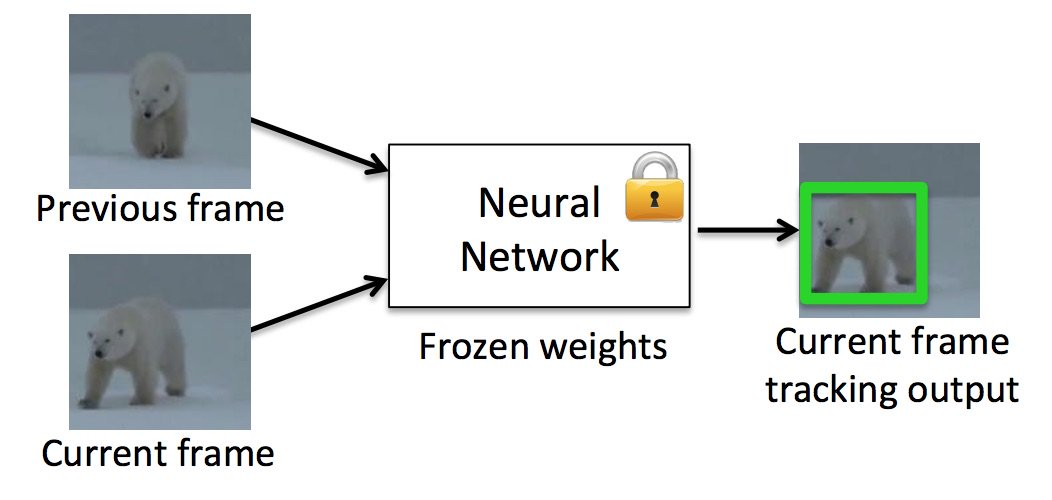
\includegraphics[width=0.7\textwidth]{object-tracking.jpg}
    \caption[Illustration of how object in two frames is tracked with a bounding box]{Illustration of how object in two frames is tracked with a bounding box\footnotemark. }
    \label{fig:object-tracking}
  \end{center}
\end{figure}

\footnotetext{
\url{https://www.learnopencv.com/goturn-deep-learning-based-object-tracking/}
}

Our hope is that by implementing an object-tracking algorithm we can use it to classify irregularities in the colonoscopy video, and then track that object in the later frames until it disappear out of frame. This will hopefully help with reducing the robustness of the network so that the classifier will not have to check every frame for irregularities. 


\subsection{Segmentation} \label{sec:segmentation}
%-----------------------------------------------------------
% Image/video segmentation. Specially related to the paper "U-Net: Convolutional Networks for Biomedical Image Segmentation" citekey UNetConvolutional15
Image segmentation is the process of partitioning a image into multiple segments of pixel, usually each segment describing some feature of the image or an entire object or class of objects. The goal of segmentation is to simplify the image and make it easier to analyze or further process. \citeauthor*{UNetConvolutional15} propose a method in the paper \citetitle*{UNetConvolutional15} \cite{UNetConvolutional15} for using a network and training strategy that relies on the strong use of data augmentation to use the available labeled samples more efficiently. This network outperform the old method of sliding-window-convolution by a great deal. They extend the "fully convolutional network" \cite{FullyConvolutional15} such that it works with very few training images and yields more precise segmentations. The way this is achieved is to supplement a contracting network by successive layers, where instead of using pooling operators, upsampling operators are used. This means that these successive layers increase the resolution of the output. The high resolution features from the contracting path are combined with the upsampled output to localize objects and with that a convolution layer can then learn to produce more precise output based on this information. 

Another important feature in this architecture is that in the upsampling portion of the network there is also large number of feature channels. These channels allow the network to pass on context information to the higher resolution layers. 

A common problem in training neural networks are too little labeled training data. This is also the case for us. We require a lot of medical data, and personell with the expertise to correctly label our data are of high demand and they usually have very little time for projects like these. This is why \citeauthor*{UNetConvolutional15} use different methods of data augmentation to generate more training data. They apply elastic deformations to the available images, and this allows the network to learn invariance to such deformations without the need to see these transformations in the annotated image corpus. Which is particular important in biomedical segmentation since deformation used to be the most common variation in tissue and realistic deformations can be simulated efficiently \cite{UNetConvolutional15}. By doing this \citeauthor*{UNetConvolutional15} were able to achieve very good results (Table \ref{tab:segmentation_results}).

\begin{table} % table:segmentation_results
  \centering
  \begin{tabular}{ l l l }
  	\hline
    Name &				PhC-U373 &			DIC-HeLa 		\\
    \hline
    IMCB-SG (2014) &	0.2669 & 			0.2935 			\\
    KTH-SE (2014) &		0.7953 & 			0.4607 			\\ 
    HOUS-US (2014) &	0.5323 & 			- 				\\ 
    second-best 2015 &	0.83 & 				0.46 			\\
    u-net (2015) &		\textbf{0.9203} & 	\textbf{0.7756} \\
    \hline
  \end{tabular}
  \caption[Segmentation results on the ISBI cell tracking challenge in 2015]{Segmentation results on the ISBI cell tracking challenge in 2015.}
  \label{tab:segmentation_results}
\end{table}


\subsection{Mapping} \label{sec:mapping}
%-----------------------------------------------------------
% Mapping of the intestine. Specially related to the paper "Deep EndoVO: A recurrent convolutional neural network (RCNN) based visual odometry approach for endoscopic capsule robots" citekey DeepEndoVO18
As mentioned in section \ref{sec:wireless_capsule_endoscopy}, a concern when processing the images taken with a WCE is not having the spatial data you get when using a normal fiber-optic endoscope. This is why \citeauthor*{DeepEndoVO18} has recently made substantial progress in converting passive capsule endoscopes to active capsule robots, enabling more accurate, precise, and intuitive detection of the location and size of the diseased areas by developing reliable real time pose estimation functionality of the capsule with RCNN's\footnote{Deep recurrent convolutional neural networks} \cite{DeepEndoVO18}. See Figure \ref{fig:deep_endovo_example} for an example.

This architecture uses inception modules for feature extraction and a RNN for sequential modelling of motion dynamics to regress the robot's orientation and position in real time. By taking multiple of RGB Depth images with timestamps it can calculate the 6-DoF pose of the capsule without the need of any extra sensors. For obtaining the depth images \citeauthor*{DeepEndoVO18} use the shape from shading (SfS) technique of \citeauthor{ShapeShading94} \cite{ShapeShading94}. This model outperforms state-of-the-art models like LSD SLAM and ORB SLAM.

\begin{figure}[h] % fig:deep_endovo_example
  \centering
  \begin{subfigure}[b]{0.4\linewidth}
    \centering
    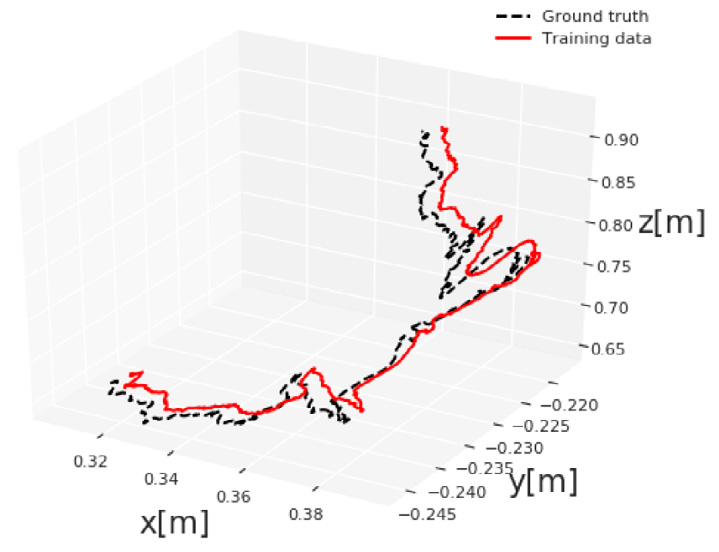
\includegraphics[width=\linewidth]{endovo_training_data}
    \caption{Training data vs ground truth.}
    \label{fig:endovo_training_data}
  \end{subfigure}
  \quad
  \begin{subfigure}[b]{0.4\linewidth}
    \centering
    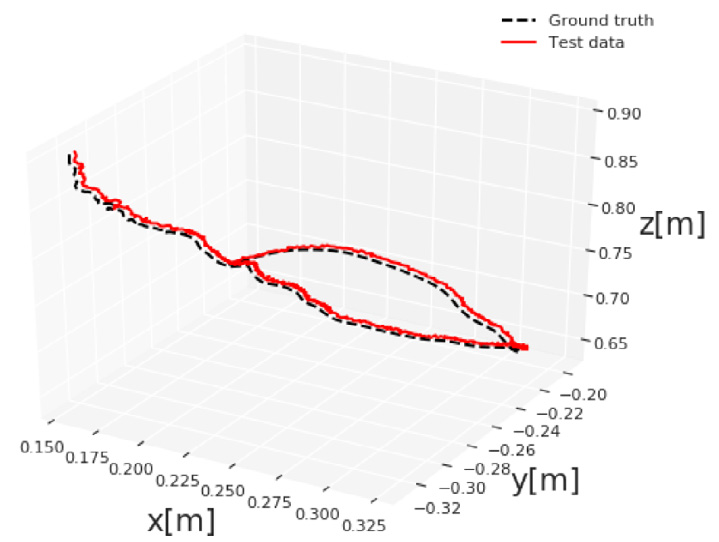
\includegraphics[width=\linewidth]{endovo_test_data}
    \caption{Test data vs ground truth.}
    \label{fig:endovo_test_data}
  \end{subfigure}
  \caption[An example of Deep EndoVO accuracy]{An example of Deep EndoVO accuracy \cite{DeepEndoVO18}.}
  \label{fig:deep_endovo_example}
\end{figure}



% ----------------------------------------------------------
\section{Summary} \label{sec:C2-summary}
% ----------------------------------------------------------


\end{document}
